
% simple alias for easier change in the future if needed
\newcommand{\mf}[1]{\mathcal{#1}}

\section{Apprentissage Profond}
\begin{frame}{Théorie de l'apprentissage profond}
Formalisme \textbf{La théorie des processus décisionnels de Markov}:
\[
    \bm{\mf{M} = \bigg\{\mf{X}, \mf{A}, \mf{R}, \mf{P}, \gamma\bigg\} }
\]

\begin{center}
    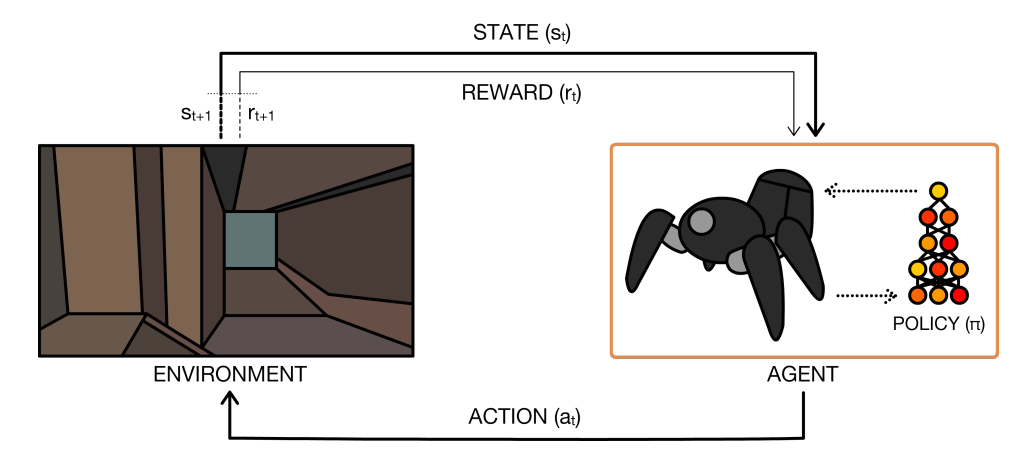
\includegraphics[scale=.2]{./reinforcementlearning/rl}
\end{center}

\end{frame}


\begin{frame}{Théorie de l'apprentissage profond}
Formalisme \textbf{La théorie des processus décisionnels de Markov}:
\[
    \bm{\mf{M} = \bigg\{\mf{X}, \mf{A}, \mf{R}, \mf{P}, \gamma\bigg\} }
\]

\begin{columns}[T] % align columns
\begin{column}{.48\textwidth}
\begin{center}
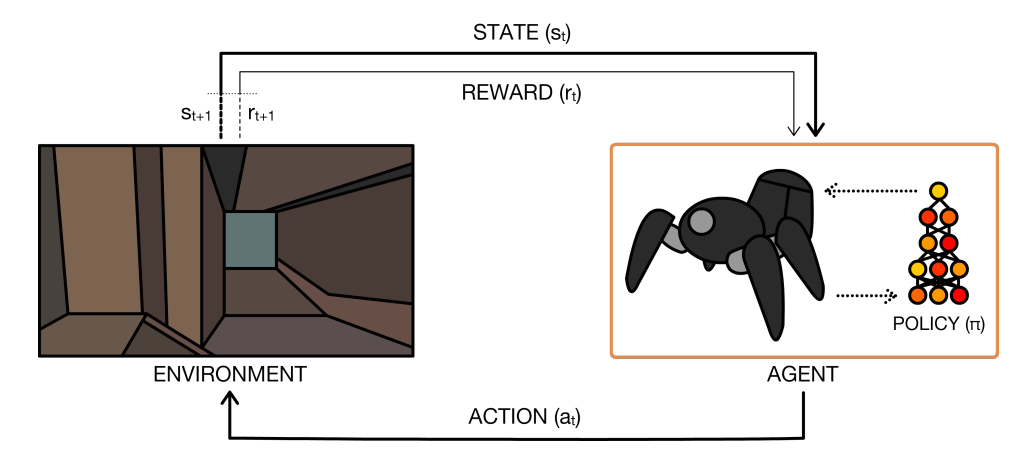
\includegraphics[scale=.14]{./reinforcementlearning/rl}
\end{center}
\end{column}%
\hfill%
\begin{column}{.68\textwidth}
\begin{itemize}
    \item \vip{Politique}\\ $\bm{\pi}$,  $\bm{a_t\:\sim\: \pi\big(\cdot, x_t\big) }$
    \item \vip{Dynamique}\\ $ x_{t+1} \:\sim\: P(\cdot, x_t, a_t) $
    \item \vip{Fonction Etat-Action}\\ $ Q^\pi(x, a) = \underset{P, \pi}{\mathbb{E}} \Big[ \underset{t}{\sum} \gamma^t r_t(x_t, a_t) \,\vert\, x_0,a_0=x,a \Big]$
\end{itemize}
\end{column}%
\end{columns}

\end{frame}
